The proteome,
the collection of different proteins used by the cell, 
is distributed over the different cellular compartments.
Proteins are found on DNA,
near ribosomes,
on membranes,
through membranes,
or become excreted.
In many Bacteria,
up to and more than a third of the proteins exit the cytoplasm,
also called the exportome.
These proteins are either embedded in the inner membrane,
reside in the cell envelope,
or are fully released in the external environment. 
In vivo,
they fulfill a variety of function like 
signalling,
transport,
and membrane biogenesis and maintenance.
Unraveling what kind of function, interactions and dynamics proteins display on their way to and inside their final location
will help to improve our general biophysical understanding of proteins and their evolutionary connections (\cite{loos2019}).
More practically, it can help improve the efficiency of recombinant protein productions,
a tool used in pharmaceutical and industrial protein production (\cite{owji2018}).
For proteins to end up in the right location,
the cell has to overcome multiple challenges.
First it needs to be able to distinguish between those protein that stay in the cytoplasm and those that have to leave it.
As cells have no internal eyes, 
recognition needs to be achieved by physical contact between internal receptors and the target protein.
This is no easy task as the cytoplasm is very crowded (Fig. \ref{fig:crowding}).
Secondly, recognised proteins need to associate with or cross through the plasmamembrane. 
Proteins are big, bulky macromolecules that need special pathways to pass the membrane.
Additionally, exported proteins tend to delay their folding.
Protein trafficking if influenced by both extrinsic factors and intrinsic factors.
Extrinsic factors include 
the cellular environment of nascent proteins,
protein concentration,
proteostatic pathways,
and translocases.
Intrinsic factors on the other hand originate from the polypeptide itself, 
but are often poorly understood:
order / disordered regions,
3D fold and motifs,
nucleotide binding domains,
and signal peptides
(\cite{loos2019}).


~\begin{figure}[h!]
  \centering
  ~\begin{subfigure}[b]{0.45\linewidth}
    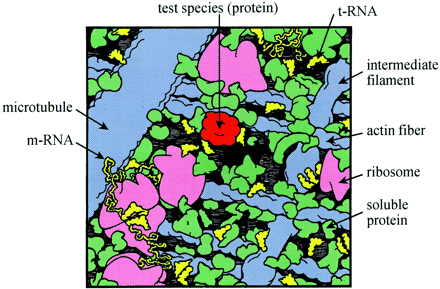
\includegraphics[width=\linewidth]
{./literature_review/subcellular_location/proteome_distribution/img/crowding_cartoon.png}
  \caption{Cartoon}
  ~\end{subfigure}
\hfill
  ~\begin{subfigure}[b]{0.48\linewidth}
    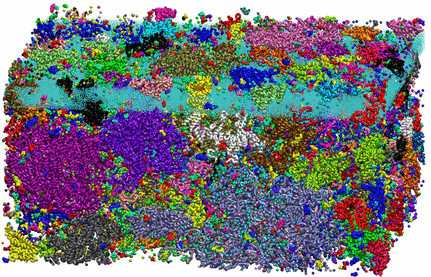
\includegraphics[width=\linewidth]
{./literature_review/subcellular_location/proteome_distribution/img/crowding_MD.png}
  \caption{Molecular dynamics simulation}
  ~\end{subfigure}
  \caption{
\textbf{Crowding in the cytoplasm.} 
\textbf{a.}
Cartoon representation of crowding in the cytoplasm at a magnification of 1,000,000.
Soluble proteins are shown in green,
RNA species in yellow,
cytoskeletal fiber in blue,
and ribosomes in pink
(from \cite{minton2001}).
\textbf{b.}
Molecular dynamics simulation of crowded cellular system.
The cytoplasm consists of proteins, RNA, metabolites, ions, and water
(from \cite{feig2017}).
}
  \label{fig:crowding}
~\end{figure}




